\section{Hasil menurut kelompok barang}\label{sec:goods}
\subsection{Mengapa berbeda dari hasil total?}
Hasil total menggabungkan banyak barang. Satu kelompok bisa membaik sementara kelompok lain memburuk. Ketika semuanya dijumlahkan, pola tersebut bisa saling menutup.

Tabel~\ref{tab:goodslr} memakai koefisien kurs pada ARDL dan koefisien depresiasi pada NARDL. Dengan definisi penelitian ini, positif mengarah pada perbaikan saat depresiasi; negatif mengarah pada pemburukan. Kode G1--G7 dijelaskan pada Tabel~\ref{tab:groups}.

Status L berarti pemeriksaan long run terpenuhi, tetapi ada catatan diagnostic tests. L+D berarti keduanya terpenuhi. Tanda -- berarti bukti long run belum cukup atau uji yang diperlukan tidak tersedia. Status ini tidak otomatis berarti koefisien kurs signifikan.

\begin{table}[!htbp]\centering\caption{Koefisien kelompok barang Indonesia--seluruh dunia}
{\small\setlength{\tabcolsep}{3pt}\renewcommand{\arraystretch}{1.15}
\begin{tabular}{p{0.05\linewidth}p{0.105\linewidth}p{0.1\linewidth}p{0.25\linewidth}p{0.1\linewidth}p{0.1\linewidth}p{0.07\linewidth}}
\toprule
\textbf{Kel.} & \textbf{Model} & \textbf{Koef.} & \textbf{CI nominal 95\%} & \textbf{p} & \textbf{BH} & \textbf{Status}\\
\midrule
G1 & ARDL & 0,865 & [-0,600; 2,330] & 0,241 & 0,463 & --\\
G1 & NARDL & 1,358 & [-0,832; 3,548] & 0,218 & 0,420 & --\\
G2 & ARDL & 2,026 & [0,198; 3,853] & 0,031 & 0,124 & L+D\\
G2 & NARDL & 4,580 & [2,301; 6,859] & \(<0{,}001\) & 0,004 & L\\
G3 & ARDL & 0,005 & [-1,248; 1,259] & 0,993 & 0,994 & --\\
G3 & NARDL & -1,621 & [-4,084; 0,842] & 0,192 & 0,380 & --\\
G4 & ARDL & -0,139 & [-6,905; 6,627] & 0,967 & 0,993 & --\\
G4 & NARDL & 7,851 & [-12,014; 27,716] & 0,431 & 0,587 & --\\
G5 & ARDL & 1,425 & [-1,754; 4,604] & 0,373 & 0,586 & --\\
G5 & NARDL & 1,589 & [-2,188; 5,365] & 0,402 & 0,578 & --\\
G6 & ARDL & -1,355 & [-1,998; -0,711] & \(<0{,}001\) & 0,004 & L+D\\
G6 & NARDL & -0,504 & [-2,145; 1,136] & 0,539 & 0,649 & --\\
G7 & ARDL & -2,040 & [-2,629; -1,451] & \(<0{,}001\) & \(<0{,}001\) & L+D\\
G7 & NARDL & -0,112 & [-1,134; 0,911] & 0,827 & 0,897 & L\\
\bottomrule
\end{tabular}
}\label{tab:goodslr}
\end{table}
\begin{figure}[!htbp]\centering
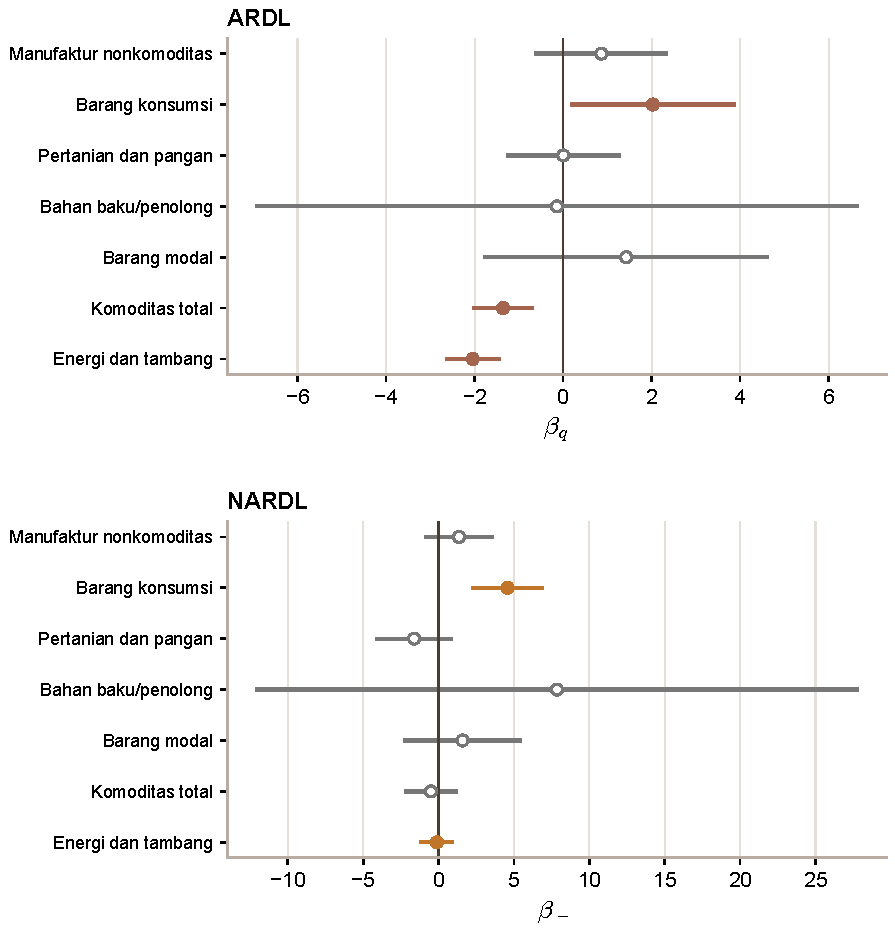
\includegraphics[width=\linewidth,height=.78\textheight,keepaspectratio]{assets/world_goods_forest.pdf}
\caption{Koefisien dan confidence interval tujuh kelompok. Cokelat: lolos pemeriksaan long run dan diagnostic tests. Emas: ada catatan model. Simbol kosong: bukti long run belum cukup.}\label{fig:goodsforest}
\end{figure}

\subsection{Komoditas total dan energi/tambang}
Pada ARDL, koefisien komoditas total sekitar $-1,355$. P-value-nya di bawah 0,001 dan BH sekitar 0,0037. Energi/tambang mempunyai koefisien sekitar $-2,040$ dengan p-value lebih kecil. Keduanya juga lolos pemeriksaan utama.

Dalam model linier ini, rupiah yang melemah berkaitan dengan memburuknya rasio perdagangan kedua kelompok. Hasilnya relevan bagi dugaan bahwa depresiasi tidak selalu memberi perbaikan.

Tetapi penyebabnya belum diketahui. Perubahan bisa berkaitan dengan harga, volume, impor, atau komposisi produk. Energi/tambang juga merupakan bagian komoditas total, sehingga keduanya bukan dua bukti yang sepenuhnya independen.

NARDL belum menguatkan kesimpulan yang sama. Koefisien depresiasi komoditas total sekitar $-0,504$ dan tidak signifikan. Joint-X test belum mendukung walaupun F dan t bounds menolak. Pada energi/tambang, koefisien sekitar $-0,112$ juga tidak signifikan, dengan catatan heteroskedasticity.

Uji asymmetry energi/tambang signifikan, tetapi koefisien depresiasinya tidak. Menguji apakah dua koefisien berbeda tidak sama dengan menguji apakah satu koefisien berbeda dari nol.

\begin{figure}[!htbp]\centering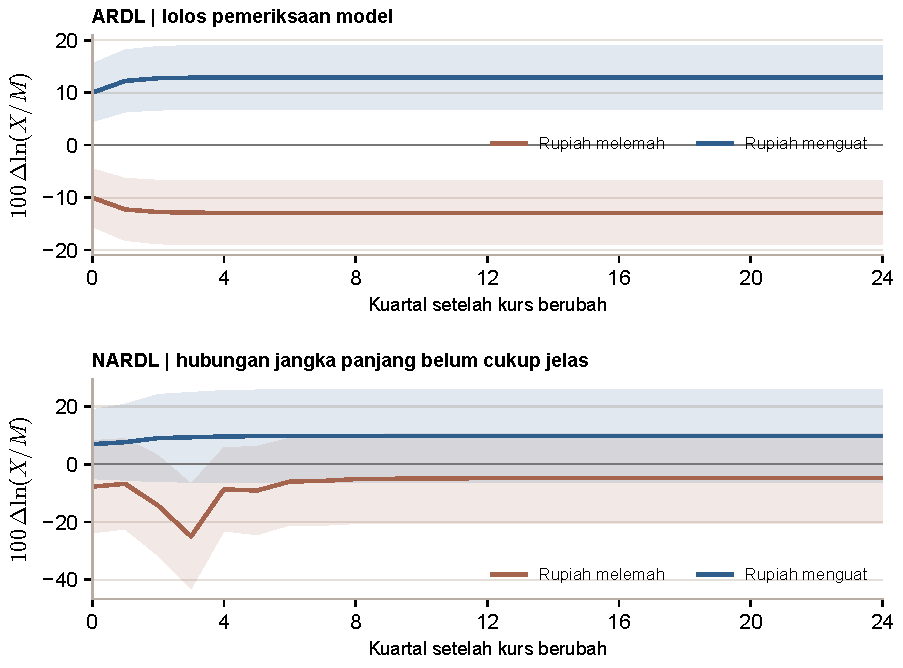
\includegraphics[width=\linewidth]{assets/response_TYPE_WLD_commodity.pdf}
\caption{Komoditas total Indonesia. ARDL mengarah pada pemburukan saat rupiah melemah; NARDL memberi hasil yang lebih tidak pasti.}\label{fig:commodity}
\end{figure}

\subsection{Manufaktur nonkomoditas}
Koefisien ARDL sekitar 0,865 dan koefisien depresiasi NARDL sekitar 1,358. Keduanya belum signifikan pada 5\%, dan pemeriksaan long run belum terpenuhi. Tanda positif belum cukup untuk mengatakan bahwa manufaktur pasti lebih diuntungkan oleh depresiasi.

Tidak signifikan juga belum berarti tidak sensitif. Confidence interval yang lebar bisa mencakup pengaruh yang cukup besar. Untuk menyatakan efek kecil, perlu batas efek yang masuk akal secara ekonomi dan pengujian khusus. Run ini belum melakukannya.

\subsection{Konsumsi, pertanian, bahan baku/penolong, dan modal}
NARDL konsumsi mempunyai koefisien sekitar 4,580 dan signifikan secara nominal maupun BH. Namun ada catatan autocorrelation, heteroskedasticity, RESET, dan CUSUMSQ. Koefisien besar tidak menghilangkan persoalan model ini.

ARDL konsumsi lolos pemeriksaan utama dan garisnya memperlihatkan pola J. Tetapi BH sekitar 0,124, dan confidence interval belum memisahkan kedua fase dengan kuat.

Pada NARDL pertanian/pangan dan modal, F dan t bounds menolak, tetapi joint-X test belum mendukung. Aturan lengkapnya belum terpenuhi. Hasil ini belum dibaca sebagai hubungan long run yang kuat.

Bahan baku/penolong mempunyai confidence interval sangat lebar dan catatan CUSUM. F/t bounds juga belum lengkap. Angka koefisien besar dalam kondisi ini lebih menunjukkan ketidakpastian daripada efek besar yang sudah pasti.

Kelompok bahan baku/penolong hanya menunjukkan penggunaan barang. Ia belum mengukur ketergantungan eksportir pada bahan impor.

\subsection{Contoh hasil yang berbeda menurut mitra}
NARDL pertanian Indonesia--Tiongkok lebih mendukung arah pemburukan. Koefisiennya sekitar $-2,037$, p-value sekitar 0,0016, dan BH sekitar 0,0148. Model juga lolos pemeriksaan utama.

Temuan tersebut berlaku pada rasio perdagangan kelompok ini dengan Tiongkok. Ia belum membuktikan bahwa seluruh ekspor pertanian Indonesia turun akibat depresiasi.

\begin{figure}[!htbp]\centering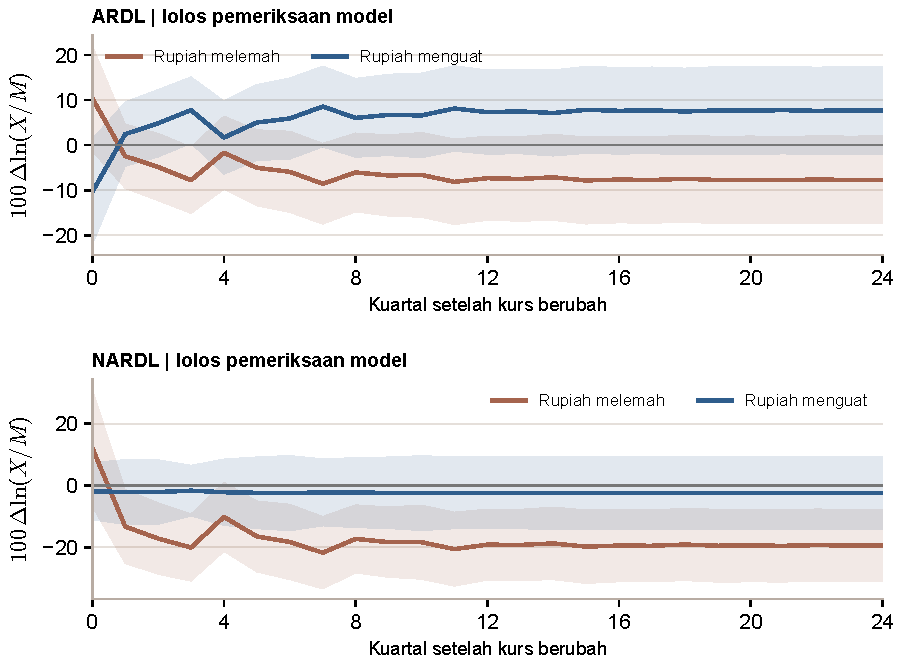
\includegraphics[width=\linewidth]{assets/response_TYPE_CHN_agriculture.pdf}
\caption{Pertanian Indonesia--Tiongkok memberi hasil berbeda dari perdagangan total dengan Tiongkok.}\label{fig:chinaagri}
\end{figure}

Sebaliknya, modal Indonesia--Korea dan konsumsi Indonesia--AS memperlihatkan pola J yang lebih jelas pada confidence interval pointwise. Ada fase awal di bawah nol dan bagian akhir di atas nol. Kedua model lolos pemeriksaan long run dan diagnostic tests.

BH modal Korea sekitar 0,104, sedangkan konsumsi AS sekitar 0,0027. Jadi, kekuatan bukti keduanya tidak persis sama. Pemilihan horizon dan model juga belum tercakup dalam satu uji simultan seluruh jalur.

\begin{figure}[!htbp]\centering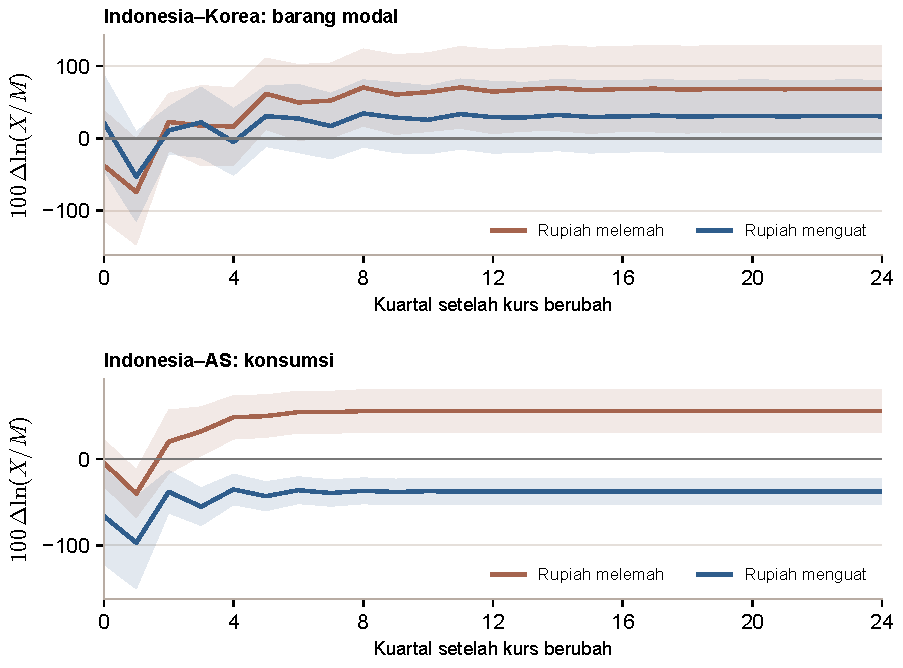
\includegraphics[width=\linewidth]{assets/J_examples.pdf}
\caption{Contoh NARDL dengan fase awal memburuk dan akhir membaik. Confidence interval berlaku per horizon, belum menjadi satu uji seluruh kurva.}\label{fig:Jexamples}
\end{figure}

Secara keseluruhan, hasil tidak memberi satu jawaban untuk semua barang dan pasar. Kita perlu melihat perbedaan tersebut tanpa langsung menyimpulkan bahwa semua komoditas tidak responsif atau selalu dirugikan.
